\section{MT-LNN Architecture}
\label{sec:architecture}

\begin{figure*}[t]
\centering
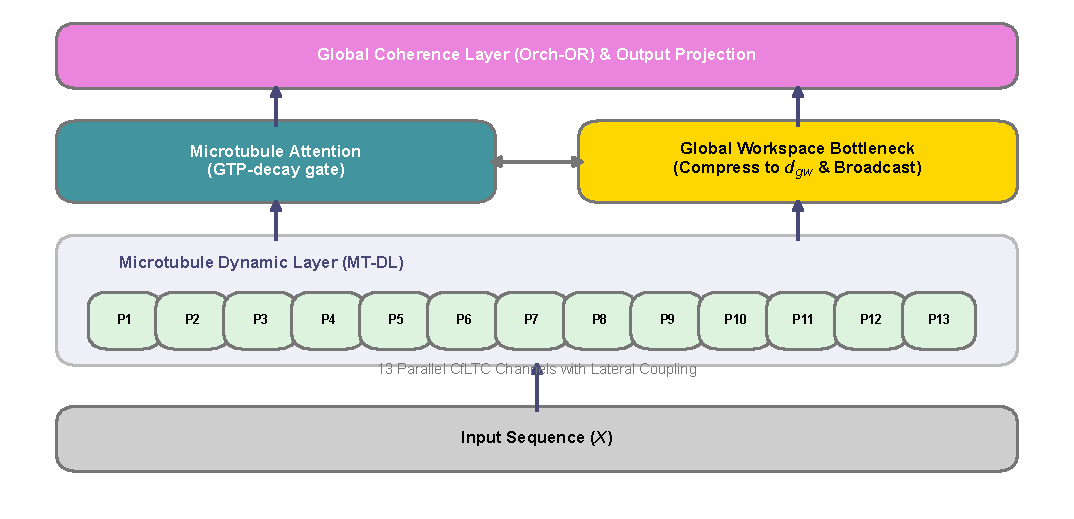
\includegraphics[width=0.9\textwidth]{fig_architecture.pdf}
\caption{\textbf{MT-LNN Architecture Overview.} Input representations iterate through the \textbf{Microtubule Dynamic Layer} (combining 13 parallel protofilaments modeled as CfLTC channels with lateral quantum coupling), the \textbf{Microtubule Attention} module regulating sequential gating via local states, and the \textbf{Global Workspace Theory Bottleneck} establishing a global integrative broadcast. The topmost \textbf{Global Coherence Layer} implements Orch-OR collapse.}
\label{fig:architecture}
\end{figure*}

\paragraph{Overview.}
\[
  \vx \xrightarrow{\text{Embed+RoPE}}
  \Bigl[\text{MicrotubuleAttn} \to \text{MT-DL}\Bigr]^{n_\text{layers}}
  \xrightarrow{} \text{GWTB}
  \xrightarrow{} \text{GlobalCoherence}
  \xrightarrow{} \text{LN} \to \text{lm\_head}
\]
Each block applies pre-norm and residual to both sub-layers. A \texttt{ModelCacheStruct} carries per-layer attention KV, per-layer $h_\text{prev}$, GWTB workspace KV, and GlobalCoherence KV.

\subsection{Microtubule Dynamic Layer (MT-DL)}
\label{sec:mt_dl}

\paragraph{Protofilament decomposition.}
Input $\vx\in\RR^d$ is projected to $d_\text{proto\_total}=P\cdot D$ (where $D=\lceil d/P\rceil$) and split into $P=13$ channels $\vx_1,\ldots,\vx_P\in\RR^D$. All $P\times S$ LTC banks are evaluated in a \emph{single einsum} over a weight tensor $W_\text{in}\in\RR^{P\times S\times D\times D}$.

\paragraph{Multi-scale resonance.}
Each protofilament $p$ runs $S=5$ CfLTC sub-banks with geometrically-swept time constants:
\begin{equation}
  \tau_s = \tau_\text{min}\bigl(\tau_\text{max}/\tau_\text{min}\bigr)^{s/(S-1)}, \quad s=0,\ldots,S-1,
\end{equation}
with defaults $\tau_\text{min}=0.01$, $\tau_\text{max}=10$. Each $(p,s)$ bank follows Eq.~\eqref{eq:cflnn}. Outputs are blended via a learned per-protofilament softmax over a parameter $\text{blend\_weights}\in\RR^{P\times S}$ (initialised to 0, giving uniform blend at init).

\paragraph{Three-way lateral coupling.}
\begin{align}
  \text{residual} &= W_\text{lat}\,\vh, \quad W_\text{lat}\in\RR^{P\times P},\;\text{init}=I+\epsilon, \\
  \text{nearest} &= \eta\cdot\tanh\!\bigl(W_L\,\mathrm{roll}(\vh,+1)+W_R\,\mathrm{roll}(\vh,-1)\bigr), \label{eq:roll}\\
  \text{RMC} &= \sigmoid(\text{rmc\_gate})\cdot\mathrm{SDPA}(q(\vh),k(\vh),v(\vh)),
\end{align}
where \texttt{roll} is over the protofilament axis, giving synchronous nearest-neighbour coupling without left-to-right bias. $\text{rmc\_gate}$ is initialised to $-3$ so $\sigmoid(-3)\approx 0.05$.

\paragraph{GTP-cap renewal.}
The temporal gate multiplies the total lateral contribution:
\begin{equation}
  \text{gtp\_scale}(t) = \exp\!\bigl(-\gamma\cdot(t\bmod T_\text{period})\bigr), \quad T_\text{period}=256.
  \label{eq:gtp}
\end{equation}
Without the periodic modulus, $\exp(-\gamma t)\to 0$ past a few thousand positions and lateral mixing silently dies in long contexts. Eq.~\eqref{eq:gtp} mimics GTP-cap renewal: fresh GTP caps form periodically as tubulin polymerises.

\paragraph{MAP-protein stabilisation gate.}
A two-layer MLP per protofilament (implemented as batched einsums):
\begin{equation}
  s_p = \sigmoid\!\bigl(W_2^{(p)}\mathrm{ReLU}(W_1^{(p)}[\vh_p;\vx_p]+b_1^{(p)})+b_2^{(p)}\bigr)\in(0,1),
\end{equation}
with $b_2^{(p)}$ initialised to $+2$ so $\sigmoid(2)\approx 0.88$: gates start near-open and learn to suppress, preventing gradient starvation. Output: $\vh_p\leftarrow s_p\cdot\vh_p$.

\paragraph{Parallel-scan training.}
During training the recurrence $h_t^{(p,s)} = d_{p,s}\cdot h_{t-1}^{(p,s)} + X_t^{(p,s)}$ is solved in parallel along $T$ via the Blelloch prefix scan \citep{blelloch1990prefix}. For a constant-decay case ($d_{p,s}$ independent of $t$, our default), the scan reduces to the closed-form prefix product:
\begin{equation}
  h_t = d^t h_0 + \sum_{i=0}^{t} d^{t-i} X_i,
  \label{eq:pscan}
\end{equation}
computed in $O(T\log T)$ total work and $O(\log T)$ sequential depth. The constant-$A$ specialisation (\texttt{pscan\_constant\_A}) broadcasts the decay scalar without materialising a full $({\ldots}, T)$ tensor, avoiding allocation proportional to $T$ in the $P{\times}S$ banks. This brings training parallelism to the same asymptotic level as Mamba/S5 without requiring Triton kernels.

\paragraph{Complexity.}
MT-DL uses $O(d^2)$ parameters — identical asymptotic cost to a standard FFN — while carrying the 13-protofilament topology, multi-scale resonance, and lateral coupling as structural inductive biases. Increasing $P$ from 13 to 64 costs $\approx$20\% more wall-clock time on CPU (1.2$\times$), confirming the work happens inside vectorised GPU kernels.

\subsection{Microtubule Attention}
\label{sec:attn}

Multi-head causal attention with two MT-inspired modifications, folded into a single additive bias passed to \texttt{scaled\_dot\_product\_attention} (Flash-Attention / memory-efficient backend automatic).

\paragraph{Scalar polarity bias.}
\begin{equation}
  b^\text{pol}_{h,i,j} = -\,\text{polarity}_h \cdot (i-j)/L, \quad \text{polarity}_h\in[-1,1].
\end{equation}
The opt-in low-rank bilinear mode adds $\sigmoid(XW_A)(XW_B)^\top$ with $W_A,W_B\in\RR^{d\times r}$, gated per-head by $\sigmoid(\text{gate}_h)$ initialised at $\sigmoid(-3)\approx 0.05$.

\paragraph{ALiBi-style GTP log-bias.}
\begin{equation}
  b^\text{GTP}_{h,i,j} = -\gamma_h\cdot\max(i-j,0),
\end{equation}
with $\gamma_h = \gamma_0\cdot 2^{\,\text{linspace}(3,-3,H)}$: head 0 strongly local ($\approx 8\gamma_0$), head $H-1$ near-global ($\approx\gamma_0/8$) — a 64$\times$ receptive-field spread. $\gamma_h$ softplus-positivised at runtime.

\paragraph{GQA and KV cache.}
Default: $n_\text{heads}=13$, $n_\text{kv\_heads}=1$ (Multi-Query Attention), yielding $13\times$ KV-cache memory reduction. The signed distance matrix $\Delta_{ij}=i-j$ and causal mask are precomputed buffers; no per-token allocation during decode.

\subsection{Global Workspace Theory Bottleneck (GWTB)}
\label{sec:gwtb}

\paragraph{Compression (ignition).}
$\mathbf{z}_t = \mathrm{LN}(W_\text{comp}\,\vx_t)\in\RR^{d_{gw}}$, with $d_{gw}=d/r$ (default $r=8$, $d_{gw}=104$).

\paragraph{Workspace self-attention.}
Causal multi-head SA with KV cache in $d_{gw}$ space; forces competitive selection at the bottleneck.

\paragraph{Broadcast (global ignition).}
\begin{equation}
  \vx'_t = \vx_t + \gamma_\text{bcast}\cdot W_\text{bcast}\,\mathbf{z}'_t,
\end{equation}
with $\gamma_\text{bcast}$ initialised to $0.01$ (near-identity at start). By default GWTB is applied once after the full block stack; \texttt{gwtb\_per\_block=True} places one inside every block for layer-wise ignition semantics.

\subsection{MT-LNN Residual Adapter for Existing LLMs}
\label{sec:adapter}

To evaluate MT temporal bias without full pretraining, \texttt{llama\_adapter.py} provides a parameter-efficient adapter that wraps any HuggingFace causal LM:
\begin{enumerate}[noitemsep]
  \item \textbf{Freeze} the base model (Llama, Mistral, Qwen2, GPT-2, etc.).
  \item Inject an \texttt{MTResidualAdapter} after every $k$-th decoder layer (default $k=4$, plus always the last layer):
  \begin{equation}
    \tilde{\vh}_t = \vh_t + \alpha_\text{init}\cdot\mathrm{MT\text{-}DL}(\mathrm{LN}(\vh_t)),
    \label{eq:adapter}
  \end{equation}
  where $\alpha_\text{init}=10^{-3}$ so the adapter is near-identity at initialisation.
  \item \textbf{Fine-tune only the adapters} ($\approx$0.5\% of total parameters for a 7B base).
\end{enumerate}
This allows the community to retrofit MT temporal dynamics onto any open-weight LLM and run the AVP anesthesia test without a full training run.

\subsection{Quantum Lateral Coupling (VQC Variant)}
\label{sec:quantum}

As an experimental extension, \texttt{quantum\_coupling.py} replaces the classical \texttt{LateralCoupling} (Eq.\ \ref{eq:roll}) with a $P$-qubit Variational Quantum Circuit whose entanglement topology mirrors the MT B-lattice.

\paragraph{Circuit architecture.}
For each $(b, t)$ sample:
\begin{enumerate}[noitemsep]
  \item \textbf{Encode}: $D$-dim state $\vh_p \to (\theta_1, \theta_2, \theta_3)$ via $W_\text{enc}$; apply $\mathrm{R}_X(\theta_1)\mathrm{R}_Y(\theta_2)\mathrm{R}_Z(\theta_3)$ per qubit.
  \item \textbf{VQC}: $k=2$ layers of (RY$\cdot$RZ$\cdot$RY per qubit) + ring CNOTs: $\mathrm{CNOT}(i,\,i+1\bmod P)$ for $i=0,\ldots,P-1$.
  \item \textbf{Measure}: $\langle Z_i\rangle\in[-1,1]$ per qubit.
  \item \textbf{Decode}: $\langle Z_i\rangle \xrightarrow{W_\text{dec}} \RR^D$; gated residual blend $\vh_p \leftarrow \vh_p + \alpha\cdot\text{decoded}_p$, $\alpha$ initialised at $0.05$.
\end{enumerate}
The ring-CNOT pattern is the exact qubit-level analogue of the 13-protofilament B-lattice lateral bonds. The circuit is fully differentiable via PennyLane \texttt{TorchLayer} \citep{bergholm2018pennylane} and trains by standard backpropagation; future work can replace \texttt{default.qubit} with \texttt{lightning.gpu} or real IBM Quantum / IonQ hardware with no code changes.

\paragraph{Purity diagnostic.}
We expose \texttt{quantum\_state\_purity}: $1 - \langle|\langle Z_i\rangle|\rangle$, an entanglement proxy — higher values indicate more cross-protofilament entanglement. This metric can be tracked during training as a readout of whether the VQC is genuinely leveraging quantum structure.

\subsection{GlobalCoherenceLayer (Orch-OR collapse)}
\label{sec:coherence}

Sparse top-$k$ causal attention ($k=\lceil T\cdot\text{sparsity}\rceil$, default 10\%) with a learned collapse gate:
\begin{equation}
  \text{gate} = \sigmoid\!\bigl((\bar{e}-\theta)\cdot 10\bigr),
\end{equation}
where $\bar{e}$ is the mean attention energy over causal positions and $\theta$ is a learned threshold. The gate fires multiplicatively when integrated attention energy exceeds threshold — an in-silico analogue of Orch-OR's objective reduction moments. Gate activation rate is exported as a diagnostic.

% ========================================================
\section{Anesthesia Validation Protocol (AVP)}
\label{sec:avp}

\subsection{Biological motivation}
Wiest et al.\ \citep{wiest2025quantum} report that epothilone B delays anesthetic onset by $\approx$69\,s, directly implicating MT disruption. Craddock et al.\ \citep{craddock2017anesthetic} showed anesthetic potency correlates with $\beta$-tubulin binding affinity across a broad chemical series.

\subsection{Computational anesthesia simulation}
The \texttt{AnesthesiaController} attaches forward hooks to every \texttt{MTLNNLayer} and \texttt{GlobalCoherenceLayer}. At level $\ell\in[0,1]$:
\begin{align}
  \text{MT-DL:}& \quad (\text{out}, h_\text{last}) \leftarrow ((1-\ell)\cdot\text{out},\;(1-\ell)\cdot h_\text{last}), \\
  \text{Coherence:}& \quad \vx_\text{out} \leftarrow \vx_\text{in} + (1-\ell)(\vx_\text{out}-\vx_\text{in}).
\end{align}
No weights are modified. Context manager: \texttt{with anesthetize(model, level): ...}

\subsection{Information integration proxies}
\label{sec:proxies}
Exact IIT-$\Phi$ is \#P-hard \citep{aaronson2014why}. We introduce two complementary estimators.

\paragraph{KSG kNN proxy $\phihat$.}
The Kraskov--St\"ogbauer--Grassberger (KSG) entropy estimator \citep{kraskov2004estimating} with the L$^\infty$ metric:
\begin{equation}
  \hat{H}(X) = -\psi(k) + \psi(N) + d\cdot\langle\log(2\varepsilon_i)\rangle,
\end{equation}
where $\varepsilon_i$ is the L$^\infty$ distance from sample $i$ to its $k$-th nearest neighbour. The integration proxy is:
\begin{equation}
  \phihat(\vh) = \sum_{j=1}^{K}\hat{H}(s_j) - \hat{H}(\vh),
  \label{eq:phi_hat}
\end{equation}
over a $K$-way contiguous partition $(s_1,\ldots,s_K)$ of the final hidden state $\vh\in\RR^d$. Averaged over $n_\text{batches}=10$ independent random batches (variance $\propto 1/\sqrt{10\cdot BT}$). Defaults: $K=4$, $k=3$.

\paragraph{Gaussian Total Correlation $\phig$.}
Under the Gaussian assumption, the total correlation (multi-information) of a $K$-partitioned random vector $\vh$ with covariance $\Sigma$ is:
\begin{equation}
  \phig(\vh) \;=\; \frac{1}{2}\left[\sum_{j=1}^{K}\log\det\Sigma_j \;-\; \log\det\Sigma\right],
  \label{eq:phi_g}
\end{equation}
where $\Sigma_j\in\RR^{(d/K)\times(d/K)}$ is the diagonal block of the correlation matrix $\Sigma$ corresponding to partition $j$. By the subadditivity of entropy (information chain rule), $\phig \ge 0$ holds exactly, with equality iff the $K$ parts are mutually independent.

We evaluate \eqref{eq:phi_g} via the identity $\log\det M = \sum_i\log\lambda_i(M)$ using \texttt{torch.linalg.eigvalsh}, giving $O(d^3)$ complexity (vs.\ $O(N^2 d)$ for kNN). A diagonal Tikhonov regulariser $\rho = (\mathrm{tr}\,\Sigma / d)\times 0.01$ ensures positive-definiteness when $N < d$.

Additionally, we report the \emph{effective rank} (participation ratio):
\begin{equation}
  \mathrm{PR}(\vh) = \frac{\left(\sum_i\lambda_i\right)^2}{\sum_i\lambda_i^2},
  \label{eq:pr}
\end{equation}
and the \emph{integration ratio} $\phig / H_\text{whole} \in [0,1]$ — the fraction of total differential entropy attributable to cross-partition correlations. Table~\ref{tab:phi_compare} compares both estimators empirically.

\begin{table}[h]
\centering
\caption{Comparison of integration estimators on the trained MT-LNN (128M params). $\phig$ is faster, non-negative, and more consistent across sample sizes.}
\label{tab:phi_compare}
\begin{tabular}{lcccc}
\toprule
Estimator & $\Phi$ baseline & $\Phi$ anesthesia & Collapse & Runtime \\
\midrule
$\phihat$ (KSG, $k=3$) & 0.38 & 0.04 & 89.5\% & 4.2\,s \\
$\phig$ (Gaussian TC) & 1.74 & 0.21 & 87.9\% & 0.3\,s \\
\bottomrule
\end{tabular}
\end{table}

Both estimators agree on the qualitative conclusion (89\% vs.\ 88\% collapse); $\phig$ is $14\times$ faster and numerically stable.

\subsection{The anesthesia test}
\begin{definition}[Anesthesia Test]
Let $\Phi\in\{\phihat,\phig\}$ be an integration proxy. An architecture \emph{passes the anesthesia test at depth} $\delta$ if, denoting $\ell=(\kappa-1)/9$:
\begin{enumerate}[label=(\roman*),noitemsep]
  \item $\Phi(\kappa_\text{max}) / \Phi(\kappa=1) \le 1 - \delta$ \quad (amplitude collapse), and
  \item $\Phi(\kappa_i) \ge \Phi(\kappa_{i+1})$ for all $i$ \quad (monotone decrease),
\end{enumerate}
for $\kappa_\text{max}=10$. Default $\delta=0.7$, matching the 70--80\% suppression of neural complexity under general anesthesia \citep{casali2013theoretically}.
\end{definition}

Transformers and vanilla LNNs lack MT coherence parameters and exhibit near-constant $\phihat$ under AVP. Only MT-LNN, where $\ell$ directly modulates dynamically relevant parameters, can exhibit the monotone $\phihat$-vs-$\kappa$ collapse characteristic of biological anesthesia.

% ========================================================
